\documentclass{article}\usepackage[]{graphicx}\usepackage[]{color}
%% maxwidth is the original width if it is less than linewidth
%% otherwise use linewidth (to make sure the graphics do not exceed the margin)
\makeatletter
\def\maxwidth{ %
  \ifdim\Gin@nat@width>\linewidth
    \linewidth
  \else
    \Gin@nat@width
  \fi
}
\makeatother

\definecolor{fgcolor}{rgb}{0.345, 0.345, 0.345}
\newcommand{\hlnum}[1]{\textcolor[rgb]{0.686,0.059,0.569}{#1}}%
\newcommand{\hlstr}[1]{\textcolor[rgb]{0.192,0.494,0.8}{#1}}%
\newcommand{\hlcom}[1]{\textcolor[rgb]{0.678,0.584,0.686}{\textit{#1}}}%
\newcommand{\hlopt}[1]{\textcolor[rgb]{0,0,0}{#1}}%
\newcommand{\hlstd}[1]{\textcolor[rgb]{0.345,0.345,0.345}{#1}}%
\newcommand{\hlkwa}[1]{\textcolor[rgb]{0.161,0.373,0.58}{\textbf{#1}}}%
\newcommand{\hlkwb}[1]{\textcolor[rgb]{0.69,0.353,0.396}{#1}}%
\newcommand{\hlkwc}[1]{\textcolor[rgb]{0.333,0.667,0.333}{#1}}%
\newcommand{\hlkwd}[1]{\textcolor[rgb]{0.737,0.353,0.396}{\textbf{#1}}}%
\let\hlipl\hlkwb

\usepackage{framed}
\makeatletter
\newenvironment{kframe}{%
 \def\at@end@of@kframe{}%
 \ifinner\ifhmode%
  \def\at@end@of@kframe{\end{minipage}}%
  \begin{minipage}{\columnwidth}%
 \fi\fi%
 \def\FrameCommand##1{\hskip\@totalleftmargin \hskip-\fboxsep
 \colorbox{shadecolor}{##1}\hskip-\fboxsep
     % There is no \\@totalrightmargin, so:
     \hskip-\linewidth \hskip-\@totalleftmargin \hskip\columnwidth}%
 \MakeFramed {\advance\hsize-\width
   \@totalleftmargin\z@ \linewidth\hsize
   \@setminipage}}%
 {\par\unskip\endMakeFramed%
 \at@end@of@kframe}
\makeatother

\definecolor{shadecolor}{rgb}{.97, .97, .97}
\definecolor{messagecolor}{rgb}{0, 0, 0}
\definecolor{warningcolor}{rgb}{1, 0, 1}
\definecolor{errorcolor}{rgb}{1, 0, 0}
\newenvironment{knitrout}{}{} % an empty environment to be redefined in TeX

\usepackage{alltt}

\setlength{\parindent}{0em}
\setlength{\parskip}{0.5em}
\IfFileExists{upquote.sty}{\usepackage{upquote}}{}
\begin{document}
\title{STAT 243 Final Project: Genetic Algorithm for Model Selection}
\author{Chris Gagne,Zicheng Huang,Yuchen Zhang,Mengying Yang}
\date{Dec 15 2017}

\maketitle



\section*{Description of Algorithm}

Our package has one main function \texttt{select()}. This applies a genetic algorithm to select the best linear model in a dataset, which contains rows as observations and columns as potential variables.

We modularized our code by breaking down the genetic algorithm into these steps and corresponding functions:
\begin{itemize}
\item (1) generating the initial population of chromosomes  \texttt{initialize()},
\item (2) calculating the fitness for that population \texttt{fitness()},
\item (3) selecting parents for breeding \texttt{selection()},
\item (4) breeding parents and choosing the next generation \texttt{nextGeneration()}. Within this function, we use \texttt{crossover()} as the genetic operator to do the actual breeding which includes doing crossover of the parent chromosomes to obtain offspring and added a small amount of randomness into the chromosome using \texttt{mutation()}.
\end{itemize}

\subsection*{Modification of Algorithm by User Input}

We also allow user input to adjust the genetic algorithm in a number of ways:

We implemented 3 ways to select parents for breeding. The first method uses fitness-rank-based probabilities to select all parents. The second method uses fitness-rank-based probabilities to choose one parent in each pair, and chooses the second parent randomly. We found that this method does better at preserving diversity in population, thus preventing early convergence. The third method uses tournament selection. This method splits the population into K groups, selects the fittest parent in each group and repeats the process until enough parents have been selected for breeding.

We also implemented a flexible generation gap -- the percentage of children replacing the parents in each generation. This had a large impact on the convergence of the algorithm to the global optimum (see examples below).

We also allow the user to specify the number of generations, the starting population size, to use glm vs. lm, and the fitness function.

\subsection*{Variable Representation}

We chose to represent our chromosomes as boolean vectors, which are used to index the data matrix. The population set of chromosomes is a matrix of these boolean chromosomes and is passed into various functions. \texttt{nextGeneration()} returns a modified version of the population set of chromosomes. We did this, rather than keep old generation chromosomes, to save memory. We do, however, store the fitness scores for each model in each generation that we can plot (see examples).

\section*{Installation}

Our package can be installed by either downloading and installing, or installing directly from github.

\begin{knitrout}
\definecolor{shadecolor}{rgb}{0.969, 0.969, 0.969}\color{fgcolor}\begin{kframe}
\begin{alltt}
\hlkwd{install}\hlstd{(}\hlstr{'GA'}\hlstd{)}
\hlkwd{install_git}\hlstd{(}\hlstr{'RPackageGroupProject/GA'}\hlstd{)}
\end{alltt}
\end{kframe}
\end{knitrout}

The package is kept in group folder: https://github.com/RPackageGroupProject/GA
The owner of the repo is: mindyyang

\section*{Documentation}

The documentation can be found by using the following:
\begin{knitrout}
\definecolor{shadecolor}{rgb}{0.969, 0.969, 0.969}\color{fgcolor}\begin{kframe}
\begin{alltt}
\hlopt{?}\hlstd{GA}\hlopt{::}\hlstd{select}
\hlopt{?}\hlstd{GA}\hlopt{::}\hlstd{crossover}
\end{alltt}
\end{kframe}
\end{knitrout}

Note that only the \texttt{select()} and \texttt{plotGA()} are directly accessible to users.

\section*{Tests}

The package can be tested using the 'testthat' package.
\begin{knitrout}
\definecolor{shadecolor}{rgb}{0.969, 0.969, 0.969}\color{fgcolor}\begin{kframe}
\begin{alltt}
\hlkwd{library}\hlstd{(}\hlstr{'testthat'}\hlstd{)}
\hlkwd{library}\hlstd{(}\hlstr{'GA'}\hlstd{)}
\hlkwd{test_package}\hlstd{(}\hlstr{'GA'}\hlstd{)}
\end{alltt}
\end{kframe}
\end{knitrout}

\section*{Example 1: basic usage}

Our package comes with many defaults, so at the minimum it can be used in one line using \texttt{select()}. All it requires is a dataset, where the first column is the predictor (y) and the rest of the columns are potential variables for the variable selection.

\begin{knitrout}
\definecolor{shadecolor}{rgb}{0.969, 0.969, 0.969}\color{fgcolor}\begin{kframe}
\begin{alltt}
\hlkwd{library}\hlstd{(}\hlstr{'GA'}\hlstd{)}
\hlstd{results}\hlkwb{<-}\hlkwd{select}\hlstd{(mtcars)}
\end{alltt}
\begin{verbatim}
## [1] "Generation:  10  Fitness:  156.134840745305"
## [1] "Generation:  20  Fitness:  156.058367373584"
## [1] "Generation:  30  Fitness:  154.32736860132"
## [1] "Generation:  40  Fitness:  154.32736860132"
## [1] "Generation:  50  Fitness:  154.32736860132"
## [1] "Generation:  60  Fitness:  154.32736860132"
## [1] "Generation:  70  Fitness:  154.32736860132"
## [1] "Generation:  80  Fitness:  154.32736860132"
## [1] "Generation:  90  Fitness:  154.32736860132"
## [1] "Generation:  100  Fitness:  154.119370868901"
## [1] "ALgorithm Ends"
\end{verbatim}
\end{kframe}
\end{knitrout}

Our function returns the best fitting model.
\begin{knitrout}
\definecolor{shadecolor}{rgb}{0.969, 0.969, 0.969}\color{fgcolor}\begin{kframe}
\begin{alltt}
\hlstd{results}\hlopt{$}\hlstd{fittestModel}
\end{alltt}
\begin{verbatim}
## 
## Call:
## model(formula = form, data = dat)
## 
## Coefficients:
## (Intercept)           wt         qsec           am  
##       9.618       -3.917        1.226        2.936
\end{verbatim}
\end{kframe}
\end{knitrout}

It also returns fitness scores for all generations, which can be plot using the our built in function \texttt{plotGA()}. The points are the fitness for individual models, and the line is the best fitness achieved at each generation.

\begin{knitrout}
\definecolor{shadecolor}{rgb}{0.969, 0.969, 0.969}\color{fgcolor}\begin{kframe}
\begin{alltt}
\hlkwd{plotGA}\hlstd{(results)}
\end{alltt}
\end{kframe}
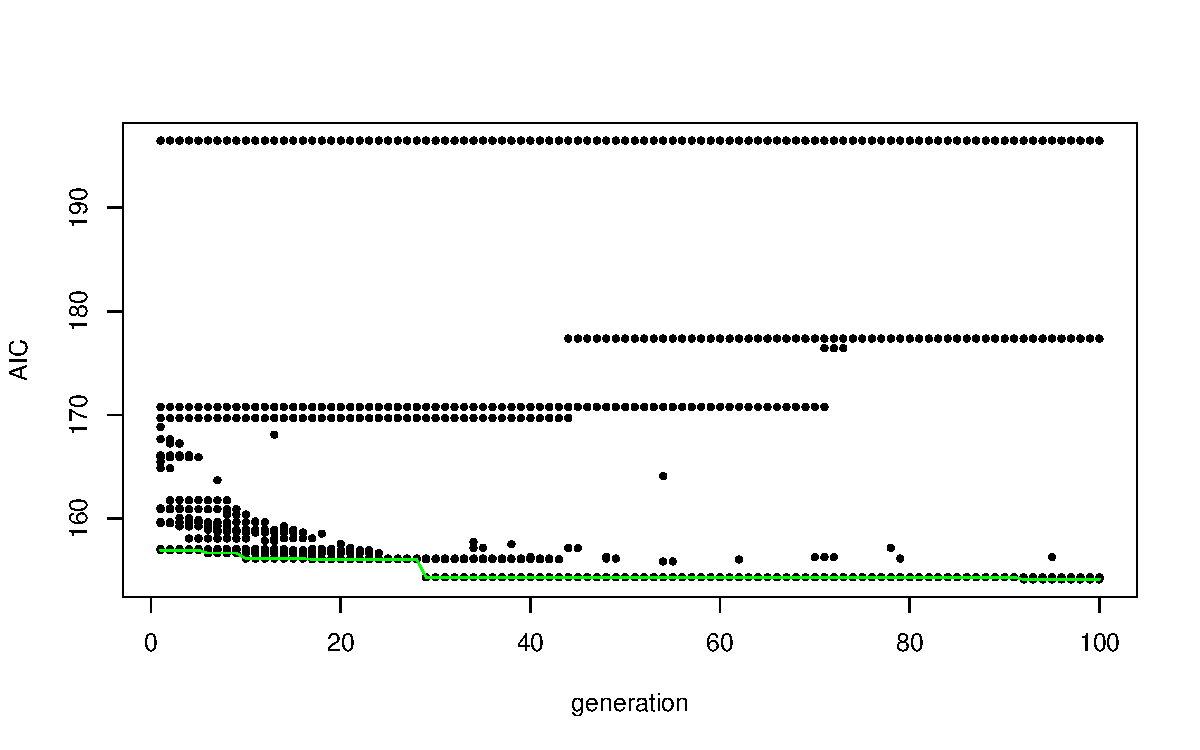
\includegraphics[width=\maxwidth]{figure/r-chunk5-1} 

\end{knitrout}

\section*{Example 2: comparison against backwards selection}

We compared the results of our model to backwards selection. Backwards selection chooses the model chooses the same model containing regressors for (wt, qseq, am). This seems to be the best model, as it's the lowest we've seen in any iteration of our algorithm. We also tried forward selection, which does not find this model.

\begin{knitrout}
\definecolor{shadecolor}{rgb}{0.969, 0.969, 0.969}\color{fgcolor}\begin{kframe}
\begin{alltt}
\hlstd{full}\hlkwb{=}\hlkwd{lm}\hlstd{(mtcars[,}\hlnum{1}\hlstd{]}\hlopt{~}\hlstd{.,} \hlkwc{data}\hlstd{=mtcars[,}\hlopt{-}\hlnum{1}\hlstd{])}
\hlkwd{step}\hlstd{(full,} \hlkwc{direction}\hlstd{=}\hlstr{"backward"}\hlstd{,}\hlkwc{trace}\hlstd{=}\hlnum{FALSE}\hlstd{)}
\end{alltt}
\begin{verbatim}
## 
## Call:
## lm(formula = mtcars[, 1] ~ wt + qsec + am, data = mtcars[, -1])
## 
## Coefficients:
## (Intercept)           wt         qsec           am  
##       9.618       -3.917        1.226        2.936
\end{verbatim}
\end{kframe}
\end{knitrout}

\section*{Example 3: user inputs}

Users can specify a number of different parameters.

\begin{knitrout}
\definecolor{shadecolor}{rgb}{0.969, 0.969, 0.969}\color{fgcolor}\begin{kframe}
\begin{alltt}
\hlkwd{library}\hlstd{(}\hlstr{'stats'}\hlstd{)}
\hlstd{userfunc}\hlkwb{<-}\hlkwa{function}\hlstd{(}\hlkwc{fit}\hlstd{,}\hlkwc{...}\hlstd{)\{}\hlkwd{return}\hlstd{(}\hlkwd{extractAIC}\hlstd{(fit,...)[}\hlnum{2}\hlstd{])\}}
\hlstd{results}\hlkwb{<-}\hlkwd{select}\hlstd{(}\hlkwc{dat}\hlstd{=mtcars,} \hlcom{# dataset}
                \hlkwc{P}\hlstd{=}\hlnum{50}\hlstd{,} \hlcom{# population size}
                \hlkwc{model}\hlstd{=glm,} \hlcom{# model lm or glm()}
                \hlkwc{numGens}\hlstd{=}\hlnum{100}\hlstd{,} \hlcom{# number of generations}
                \hlkwc{G}\hlstd{=}\hlnum{0.25}\hlstd{,} \hlcom{# generation gap}
                \hlkwc{method}\hlstd{=}\hlnum{2}\hlstd{,} \hlcom{# parent selection method}
                \hlkwc{K}\hlstd{=}\hlnum{2}\hlstd{,} \hlcom{# number of groups for tournament selection}
                \hlkwc{fitnessFunction}\hlstd{=userfunc,} \hlcom{#user defined fitness}
                \hlkwc{verbose}\hlstd{=}\hlnum{FALSE}\hlstd{,} \hlcom{# whether to print results}
                \hlstd{)}
\end{alltt}
\begin{verbatim}
## [1] "ALgorithm Ends"
\end{verbatim}
\begin{alltt}
\hlstd{results}\hlopt{$}\hlstd{fittestModel}
\end{alltt}
\begin{verbatim}
## 
## Call:  model(formula = form, data = dat)
## 
## Coefficients:
## (Intercept)           wt         qsec           am  
##       9.618       -3.917        1.226        2.936  
## 
## Degrees of Freedom: 31 Total (i.e. Null);  28 Residual
## Null Deviance:	    1126 
## Residual Deviance: 169.3 	AIC: 154.1
\end{verbatim}
\end{kframe}
\end{knitrout}

We can plot this as well. Notice that with a smaller generation gap, the population maintains variance for longer.
\begin{knitrout}
\definecolor{shadecolor}{rgb}{0.969, 0.969, 0.969}\color{fgcolor}\begin{kframe}
\begin{alltt}
\hlkwd{plotGA}\hlstd{(results)}
\end{alltt}
\end{kframe}
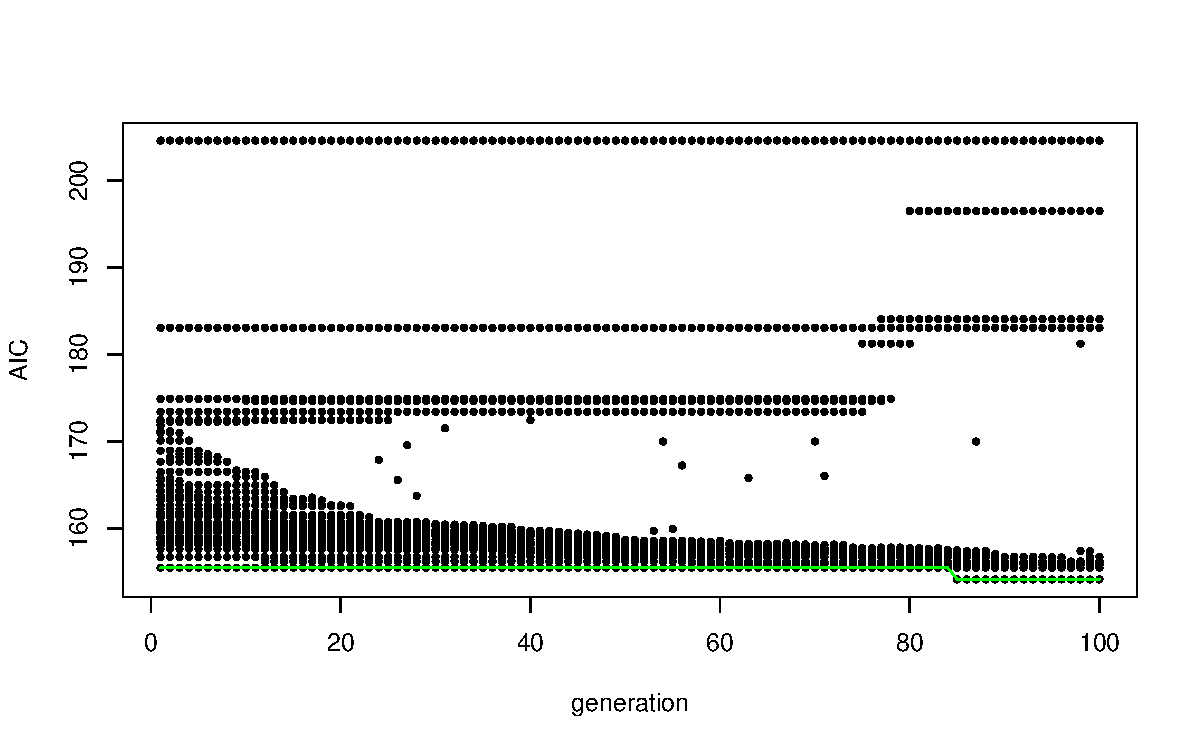
\includegraphics[width=\maxwidth]{figure/r-chunk6b-1} 

\end{knitrout}

\section*{Example 4: early convergence}

A big difference in our algorithm is the generation Gap. With too high of a generation gap, the algorithm often converges to a local minimum. We considered adjusting the mutation rate and not allowing duplicate parents. These should both help.

\begin{knitrout}
\definecolor{shadecolor}{rgb}{0.969, 0.969, 0.969}\color{fgcolor}\begin{kframe}
\begin{alltt}
\hlstd{results}\hlkwb{<-}\hlkwd{select}\hlstd{(}\hlkwc{dat}\hlstd{=mtcars,}\hlkwc{G}\hlstd{=}\hlnum{.8}\hlstd{,}\hlkwc{verbose}\hlstd{=}\hlnum{TRUE}\hlstd{)}
\end{alltt}
\begin{verbatim}
## [1] "Generation:  10  Fitness:  155.657784908588"
## [1] "Generation:  20  Fitness:  155.657784908588"
## [1] "Generation:  30  Fitness:  155.657784908588"
## [1] "Generation:  40  Fitness:  155.657784908588"
## [1] "Generation:  50  Fitness:  154.563104963084"
## [1] "Generation:  60  Fitness:  154.563104963084"
## [1] "Generation:  70  Fitness:  154.563104963084"
## [1] "Generation:  80  Fitness:  154.563104963084"
## [1] "Generation:  90  Fitness:  154.563104963084"
## [1] "Generation:  100  Fitness:  154.563104963084"
## [1] "ALgorithm Ends"
\end{verbatim}
\begin{alltt}
\hlstd{results}\hlopt{$}\hlstd{fittestModel}
\end{alltt}
\begin{verbatim}
## 
## Call:
## model(formula = form, data = dat)
## 
## Coefficients:
## (Intercept)           wt         qsec           am         carb  
##     12.8972      -3.4343       1.0191       3.5114      -0.4886
\end{verbatim}
\end{kframe}
\end{knitrout}

You can see that most of the population converged to the local minimum.
\begin{knitrout}
\definecolor{shadecolor}{rgb}{0.969, 0.969, 0.969}\color{fgcolor}\begin{kframe}
\begin{alltt}
\hlkwd{plotGA}\hlstd{(results)}
\end{alltt}
\end{kframe}
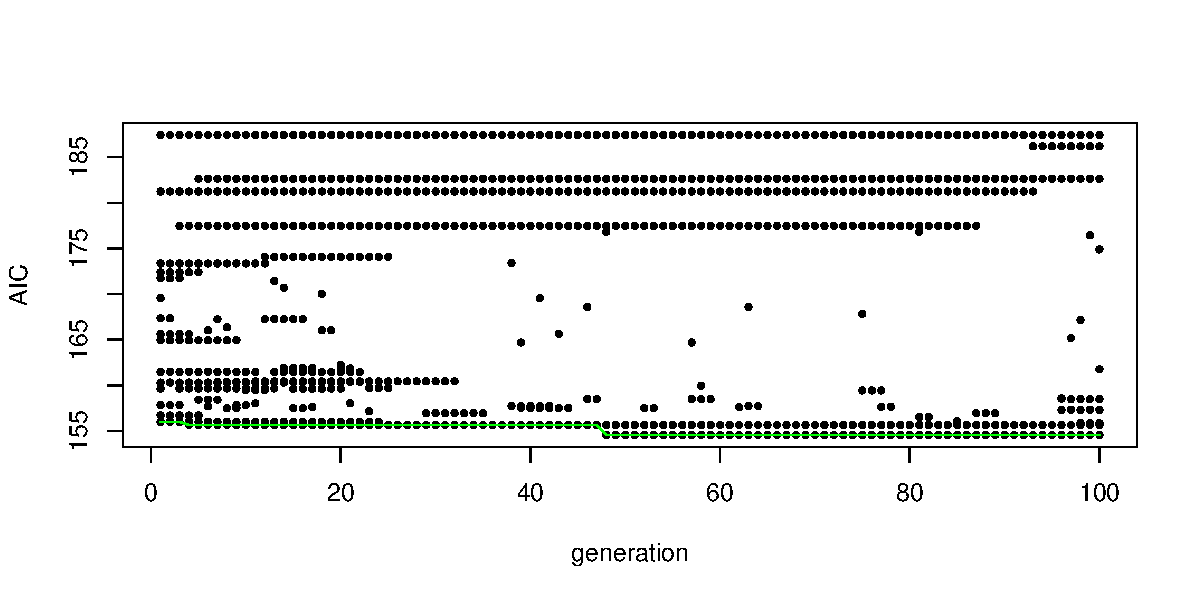
\includegraphics[width=\maxwidth]{figure/r-chunk16b-1} 

\end{knitrout}


\section*{Contributions of Team Members}

The project consisted of the following components. We put who contributed to each part in parentheses:
\begin{itemize}
\item design of algorithm (all members)
\item select function (Chris and Zicheng)
\item parent selection (Yuchen and Mengying)
\item crossover (Yuchen and Mengying)
\item other function (all members)
\item package organization (Chris)
\item tests (all members)
\item pdf document (Chris and Zicheng)
\end{itemize}


\end{document}
